\documentclass[12pt]{article}

\usepackage{units}
\usepackage{graphicx}

\setlength{\oddsidemargin}{0in}
\setlength{\evensidemargin}{0in}
\setlength{\textwidth}{6.5in}
\setlength{\topmargin}{-.3in}
\setlength{\textheight}{9in}
\pagestyle{empty}

\graphicspath{{images/}}

\usepackage{cleveref}
\usepackage{float}
%\crefformat{equation}{equation (#2#1#3)} % this is to remove the space...
\Crefname{equation}{Equation}{Equations}
\crefname{equation}{Eq.}{Equations}

\crefformat{section}{\S#2#1#3}
\crefformat{subsection}{\S#2#1#3}
%\crefname{subsection}{\S}{\S}
\Crefname{section}{Section}{Sections}
\Crefname{subsection}{Section}{Sections}

\crefname{figure}{Fig.}{Figures}
\Crefname{figure}{Figure}{Figures}

%----------------------------------------------------------------------------------------
%	TITLE SECTION
%----------------------------------------------------------------------------------------

\title{	
\normalfont \Large 
\textsc{Campus Safety and Security\\Process Book} \\ [10pt] 
Mohsen Abbasi\footnote{UID: u1011952, Email: m.abbasi@utah.edu} \\ 
Amir Biglari\footnote{UID: u0613945, Email: amir.biglari@utah.edu}\\
Waiming Tai\footnote{UID: u1008421, Email: u1008421@utah.edu}
}
\date{}

\begin{document}

\maketitle
\noindent

\section{Overview and Motivation}
Choosing an institution in USA and even choosing an appropriate US state or city is a major decision for students and their families. Along with academic, financial and 
geographic considerations, the safety of campus is a vital concern. This work tries to investigate the campus safety by considering on-campus crime records all over the US. 

Students can better compare the crime records in US States and universities using the visualizations in this work. In addition, social scientists can use this visualized data to find in what universities and states there are more problems related to crimes. They can also see the record of different types and categories of crimes separately at different schools and location. This may help them find if there is any relation between an specific crime type/category to its geographic location.

\section{Questions to answer}
By visualizing this data set, we have a few questions to answer and objectives in mind:
\begin{itemize}
\item Answering basic questions such as: 
\begin{enumerate}
\item Which states have the safest campuses across the United States? 
\item Find the safest and unsafest schools campuses across the United States.
\item Find the safest and unsafest schools campuses across a specific state.
\item Which schools are facing some specific type of criminal activities more than the others? 
\item Which schools are similar considering a particular type of crime?   
\item Is there any relation between a specific type of criminal activity on-campuses with their geographic locations?
\item Which type of crime has been the most threat to the students at a specific year at different locations?
\item How does the crime rate has changed in time?


\end{enumerate}
\item We're also interested in comparing different schools in details and finding out what types of crimes plays a more significant role in threatening the safety of students of a school.
\item Categories such as criminal offenses, disciplinary actions,  hate crimes and violence against women are included in the data set. As a future work or continuation of this work, it will be interesting to combine this data set with other ones containing demographic information, GDP and such for different states and look for correlations between the crime rates and these attributes. 

\end{itemize}

\section{Data}
The datasets that we worked with is about ``The Campus Safety and Security". The raw data for this work can be accessed from ``http://ope.ed.gov/campussafety/\#/". This data set is so inclusive and contains the information about all the universities across the US with all of their campuses inside or outside the US, all institution sectors, and all programs.  This data can also be sliced according to different school sizes. This database also includes information about crimes related to on-campus, on-campus housing, non-campus, public properties, and Reported by locals and state police. It has the records related to the years between 2001 and 2014.

However, in order to reduce the volume of the data and also considering the more important, and more popular schools which are more appropriate for our works, we filter the data before downloading it from the website. 

For this work, we only considered the crimes conducted on-campus between 2001 and 2014. We filtered down the institution sectors to 1) Public, 4-year or above, 2) Private nonprofit, 4-year or above, ans 3)Private for-profit, 4-year or above. We also filtered the data with respect to institution enrollment (that shows the institution size) and only considered the schools with more that 10000 students.

The crimes covered in the data set are categorized into criminal offenses such as theft, disciplinary actions such as criminal actions, hate crimes, VAWA offenses and others. Disciplinary actions has categories of illegal weapons possession, drug law violations, and liquor law violations. Criminal offenses includes murder/non-negligent manslaughter, negligent manslaughter, sex offenses-forcible, rape, fondling, sex offenses-nonforcible, incest, statutory rape, robbery, aggravated assault, burglary, motor vehicle theft, and arson. Hate crimes has 150 sub-categories and violent against women includes domestic violence, dating violence, stalking.

Fortunately (for the sake of safety on campuses), "The Campus Safety and Security" data set is a sparse one (there are many zero values in each record). We considered all of those entries as 0. Also, note that the record related to violence against women has only conducted at 2014. We copied this record to all the previous years for better visualization.

The database can provide all the data for universities together, or separated with respect to states. But it won't generate a data that includes state tags. Therefore, for data related to the states, we needed to process the data and combine some of it. Also for each of the four categories, we needed to calculated their sum from their subcategories.

\section{Design Evolution and Related Works}

There are three phenomenons we would like to study and visualize:
\begin{enumerate}
\item The crime statistics for different institutes in each state. Also, see how these statistics have changed over time.
\item Analyze the statistics by choosing a specific type of crime. For each type of crime, the trend for different categories of that crime over time will be shown in graphs.
\item Comparing the crime statistics between different schools. By choosing two or more schools, different types of crime would be compared.
\end{enumerate}
The following are the designs we'd like to consider:\\

\subsection{Must-Have and Optional Features:}
We should be able to easily observe the crime statistics for different schools in each state and be able compare them. We should be able to see how different states are compared to each other in terms of crime statistics in their schools. Also, we should be able to see how these statistics have changed over the years.\\
As mentioned in the objectives, we'd like to combine this data set with other ones containing demographic information, GDP and such for different states and look for correlations between the crime rates and these attributes.

\subsection{Crime statistics in each state:} 
This design would be to display the map of the United States. Here each state is colored using a gradient color map that uses saturation with respect to the crime number per students in that state. The map is broken down by states where each one is selectable. There is also a time line bar that can be adjusted to the desired year. Beside the map there would be a line chart showing the trend of the change in the number of different types of crimes in US universities in time (\cref{fig:p1-overall}). By selecting a specific type you would be able to see a bar plot showing the amount of crimes for different crime categories of that type (\cref{fig:p1-1}). By hovering over a state you can see a general information about it (\cref{fig:p1-2}). By choosing a state, line chart and the barchart beside the map would get updated with respect to that specific state. The general crime statistics would also be displayed below the map on a line chart in which each line represents a school in the selected state (\cref{fig:p1-3}) and by hovering over the lines you can see the schools names (\cref{fig:p1-4}). Also, when a line in the line chart is selected, the detail breakdown of different types of crimes would be displayed on a stack bar chart (\cref{fig:p1-5}). By selecting each chunk of the stack bar chart, you will get another stack bar chart for the categories of that crime type for the specific school (\cref{fig:p1-6}). There would be two search boxes to search any two schools and compare their crime statistics. By selecting a pair of schools and do hitting the compare button the user will get a new view which compares the school crime statistics in line charts and bar charts.


\begin{figure}[tbph]
   \centering{}
	       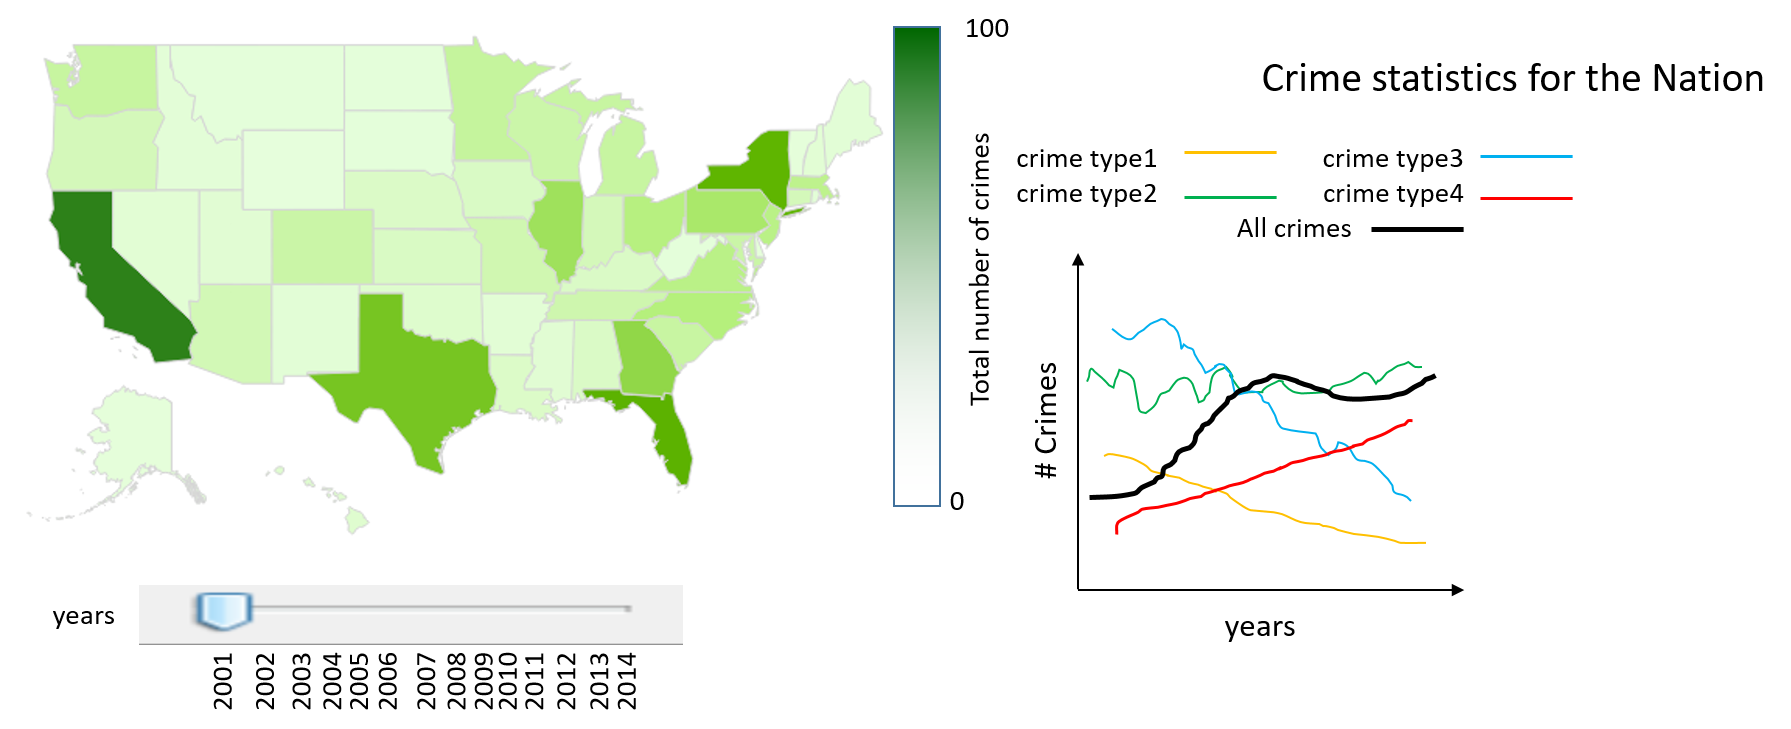
\includegraphics[width=6in]{prot1-overall}           
\caption{}
\label{fig:p1-overall}
\end{figure}

\begin{figure}[tbph]
   \centering{}
	       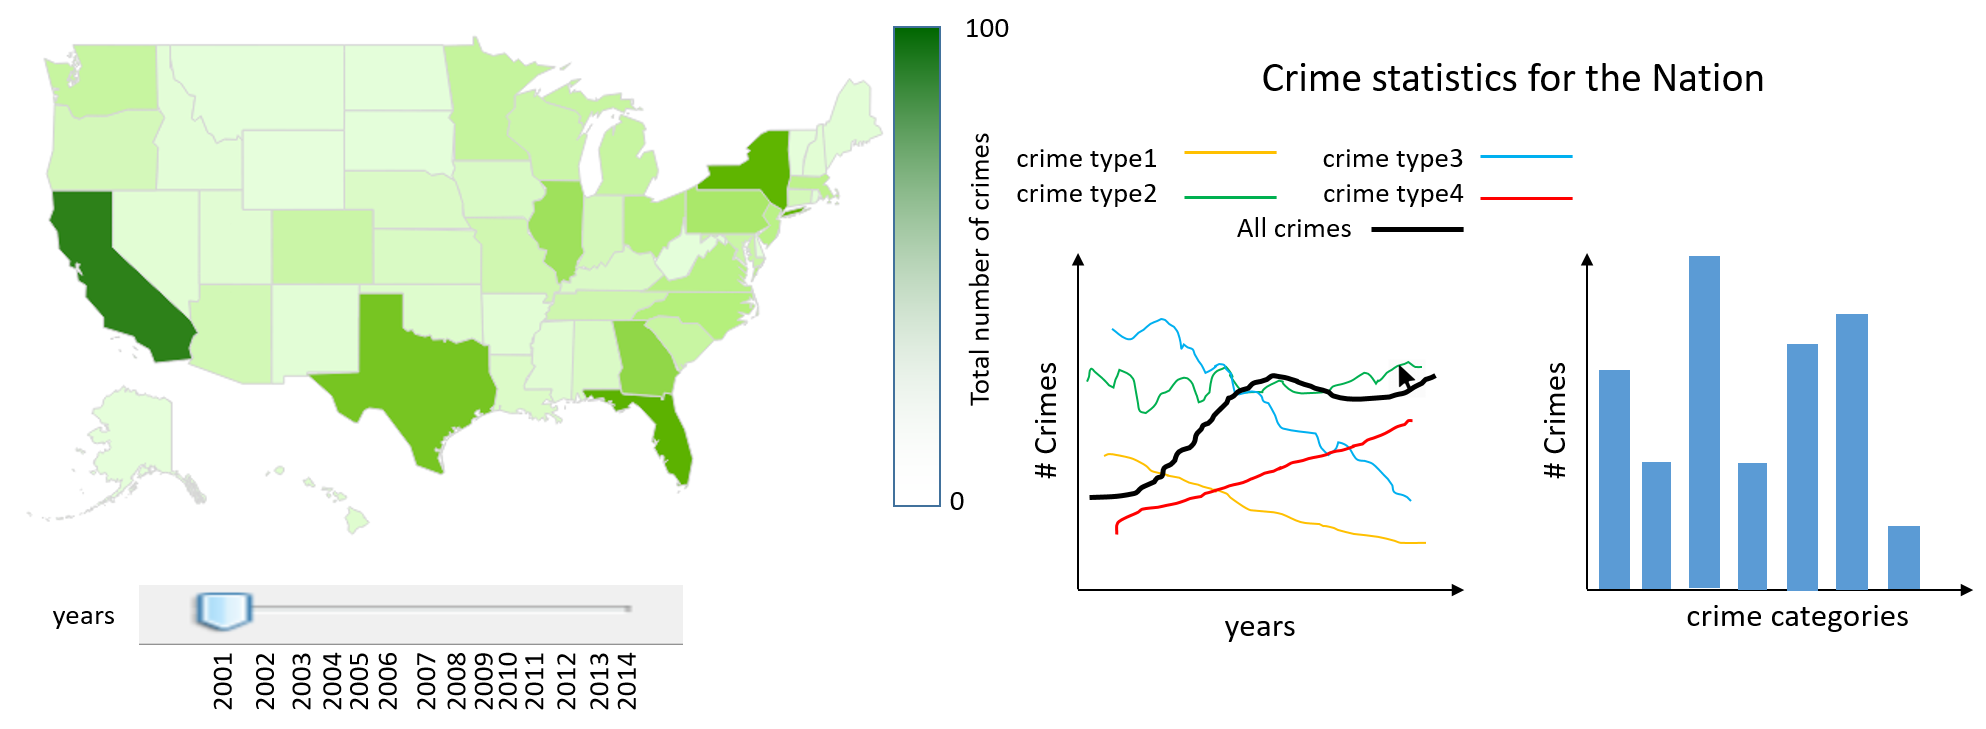
\includegraphics[width=6in]{prot1-1}           
\caption{}
\label{fig:p1-1}
\end{figure}

\begin{figure}[tbph]
   \centering{}
	       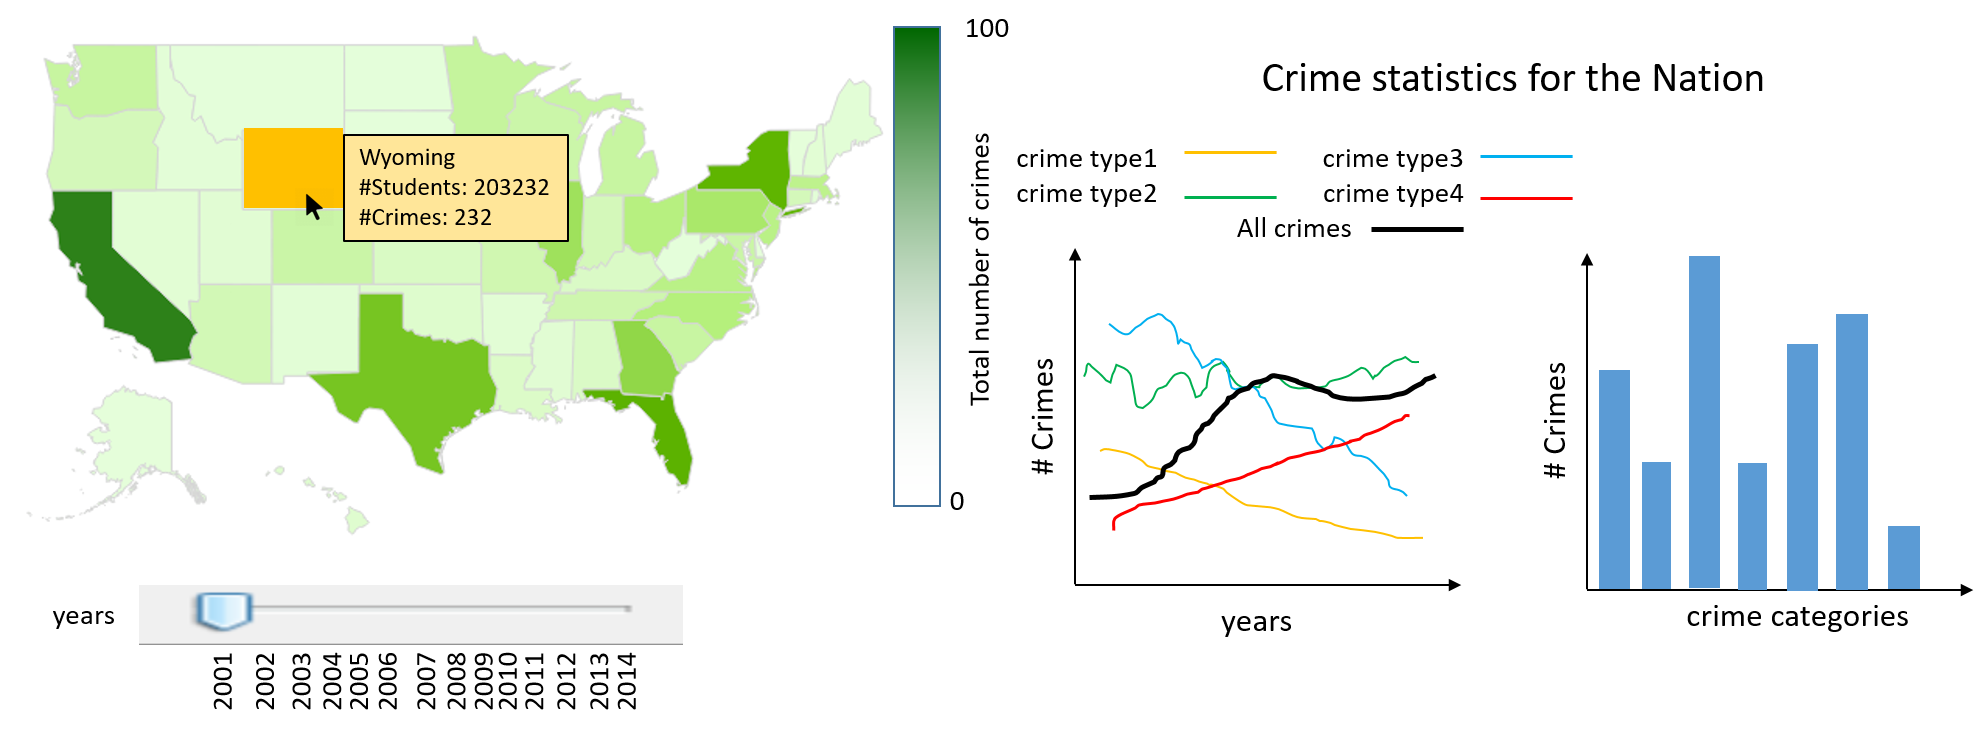
\includegraphics[width=6in]{prot1-2}           
\caption{}
\label{fig:p1-2}
\end{figure}

\begin{figure}[tbph]
   \centering{}
	       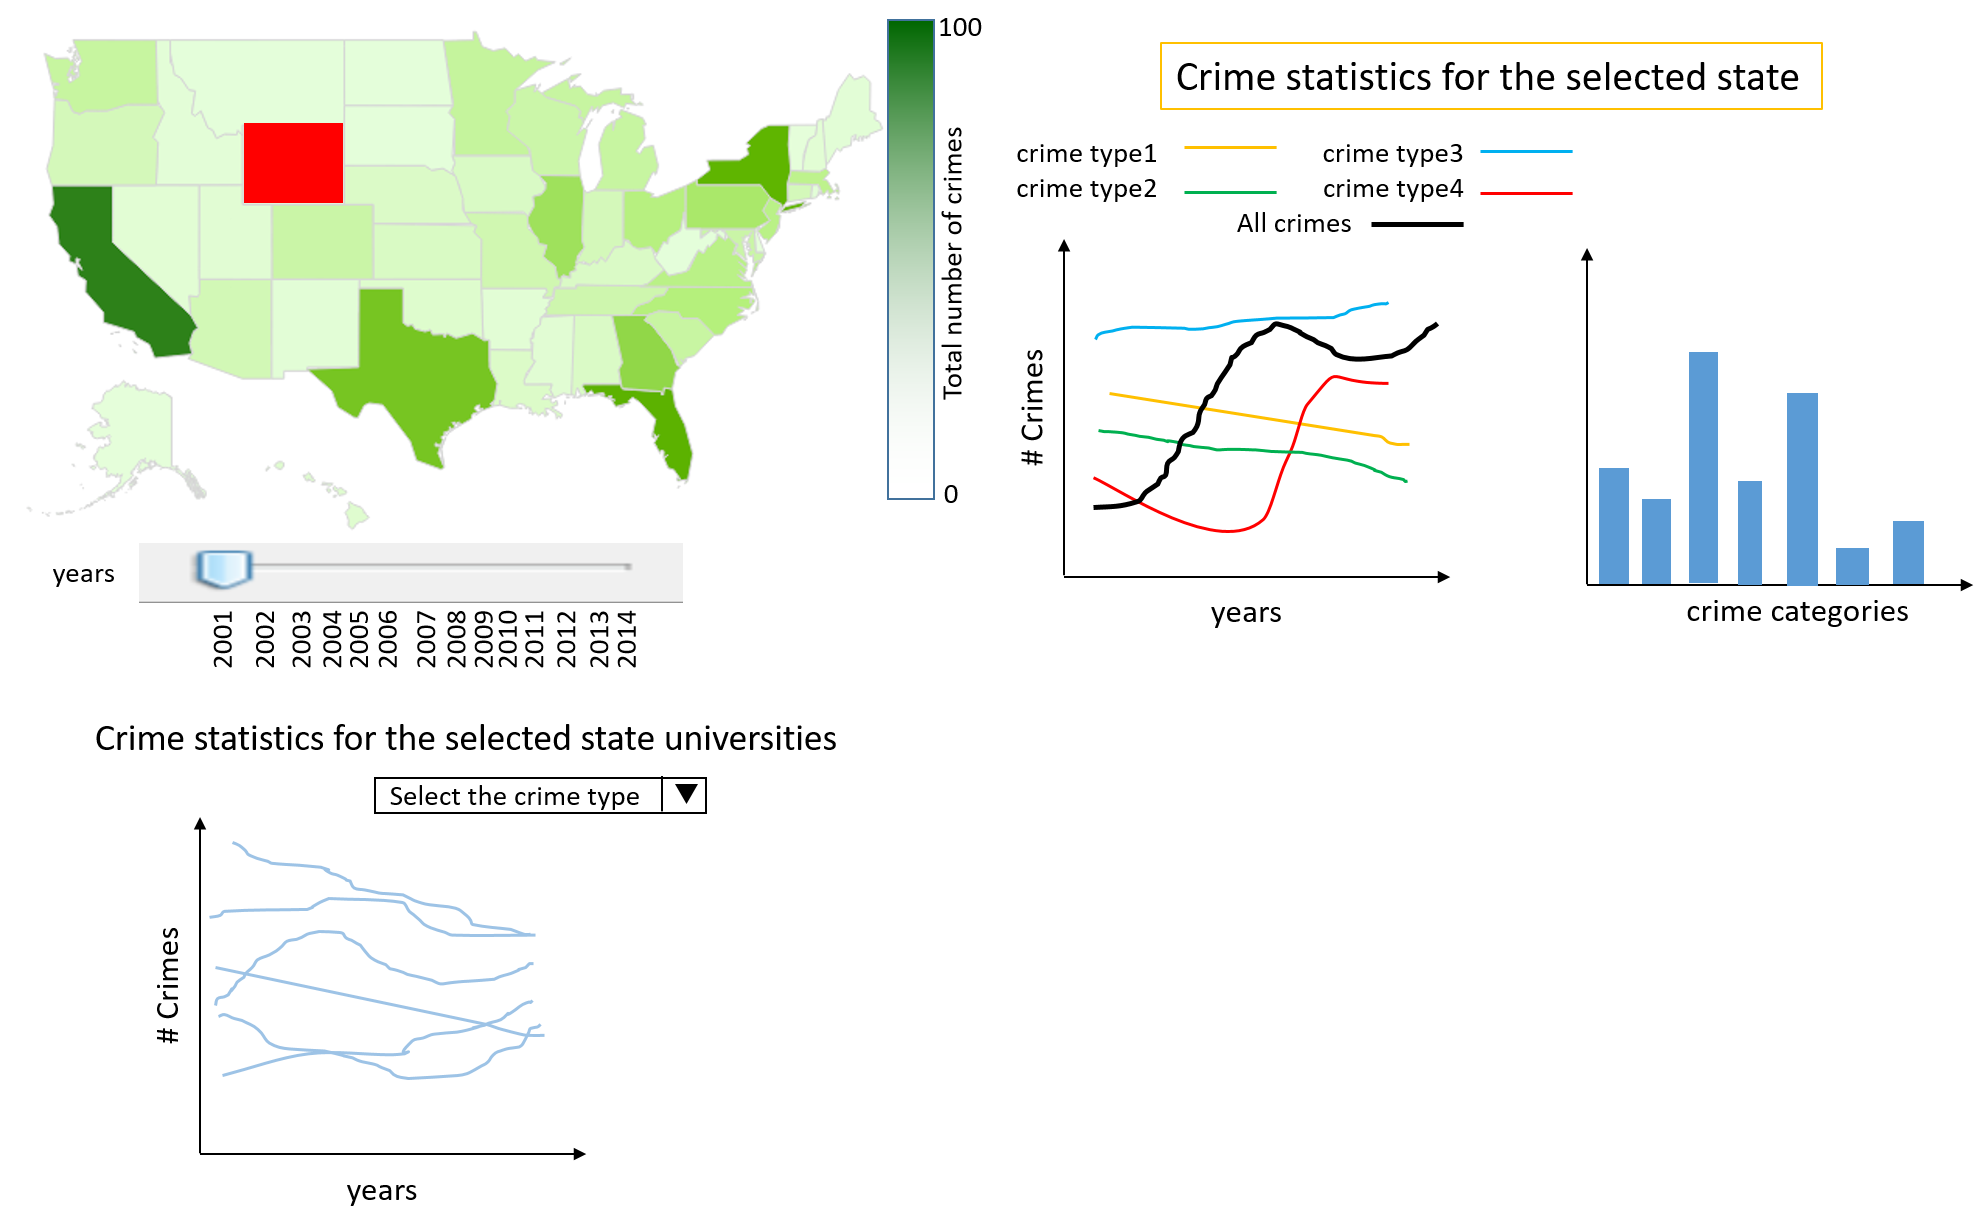
\includegraphics[width=6in]{prot1-3}           
\caption{}
\label{fig:p1-3}
\end{figure}

\begin{figure}[tbph]
   \centering{}
	       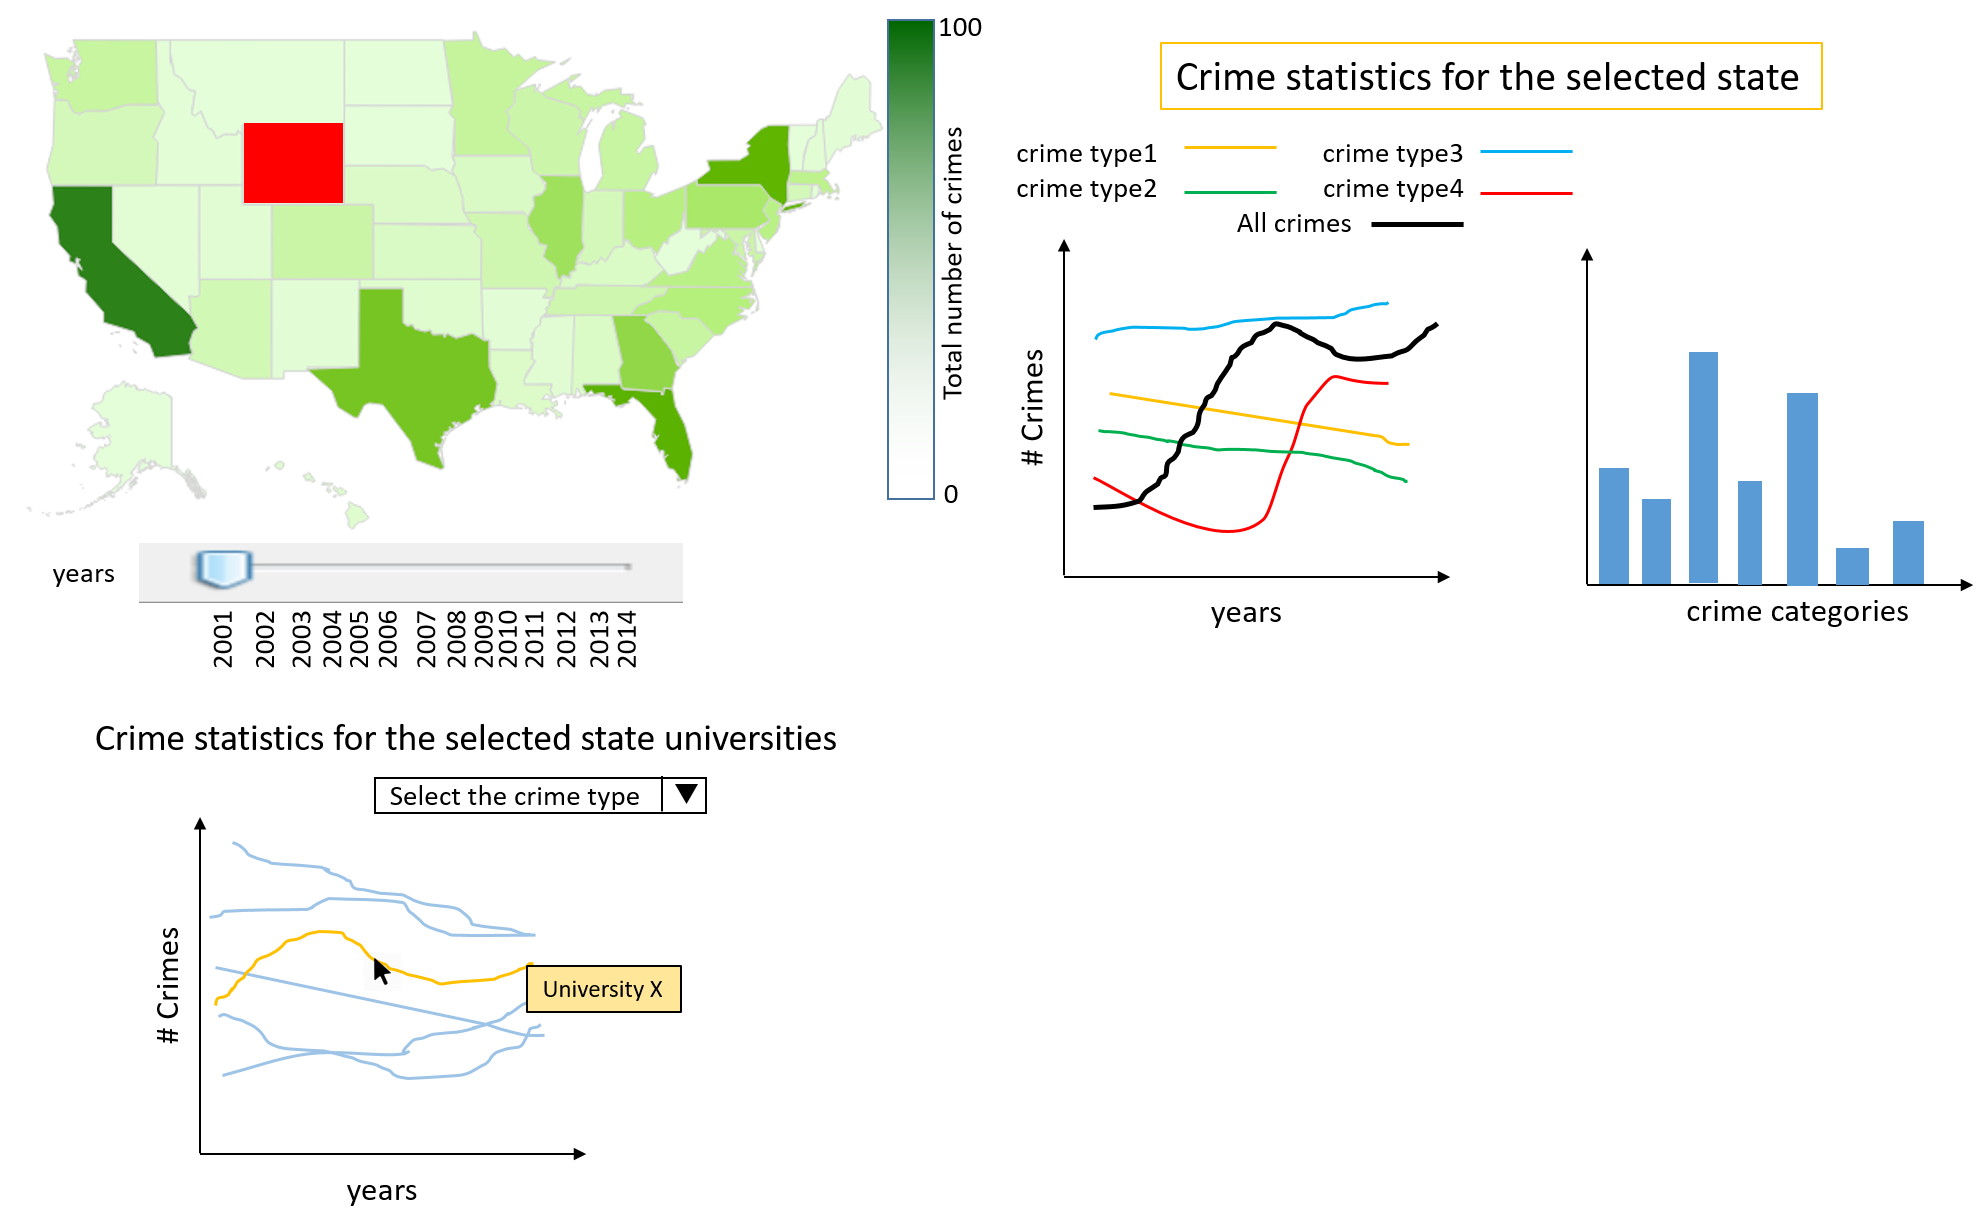
\includegraphics[width=6in]{prot1-4}           
\caption{}
\label{fig:p1-4}
\end{figure}

\begin{figure}[tbph]
   \centering{}
	       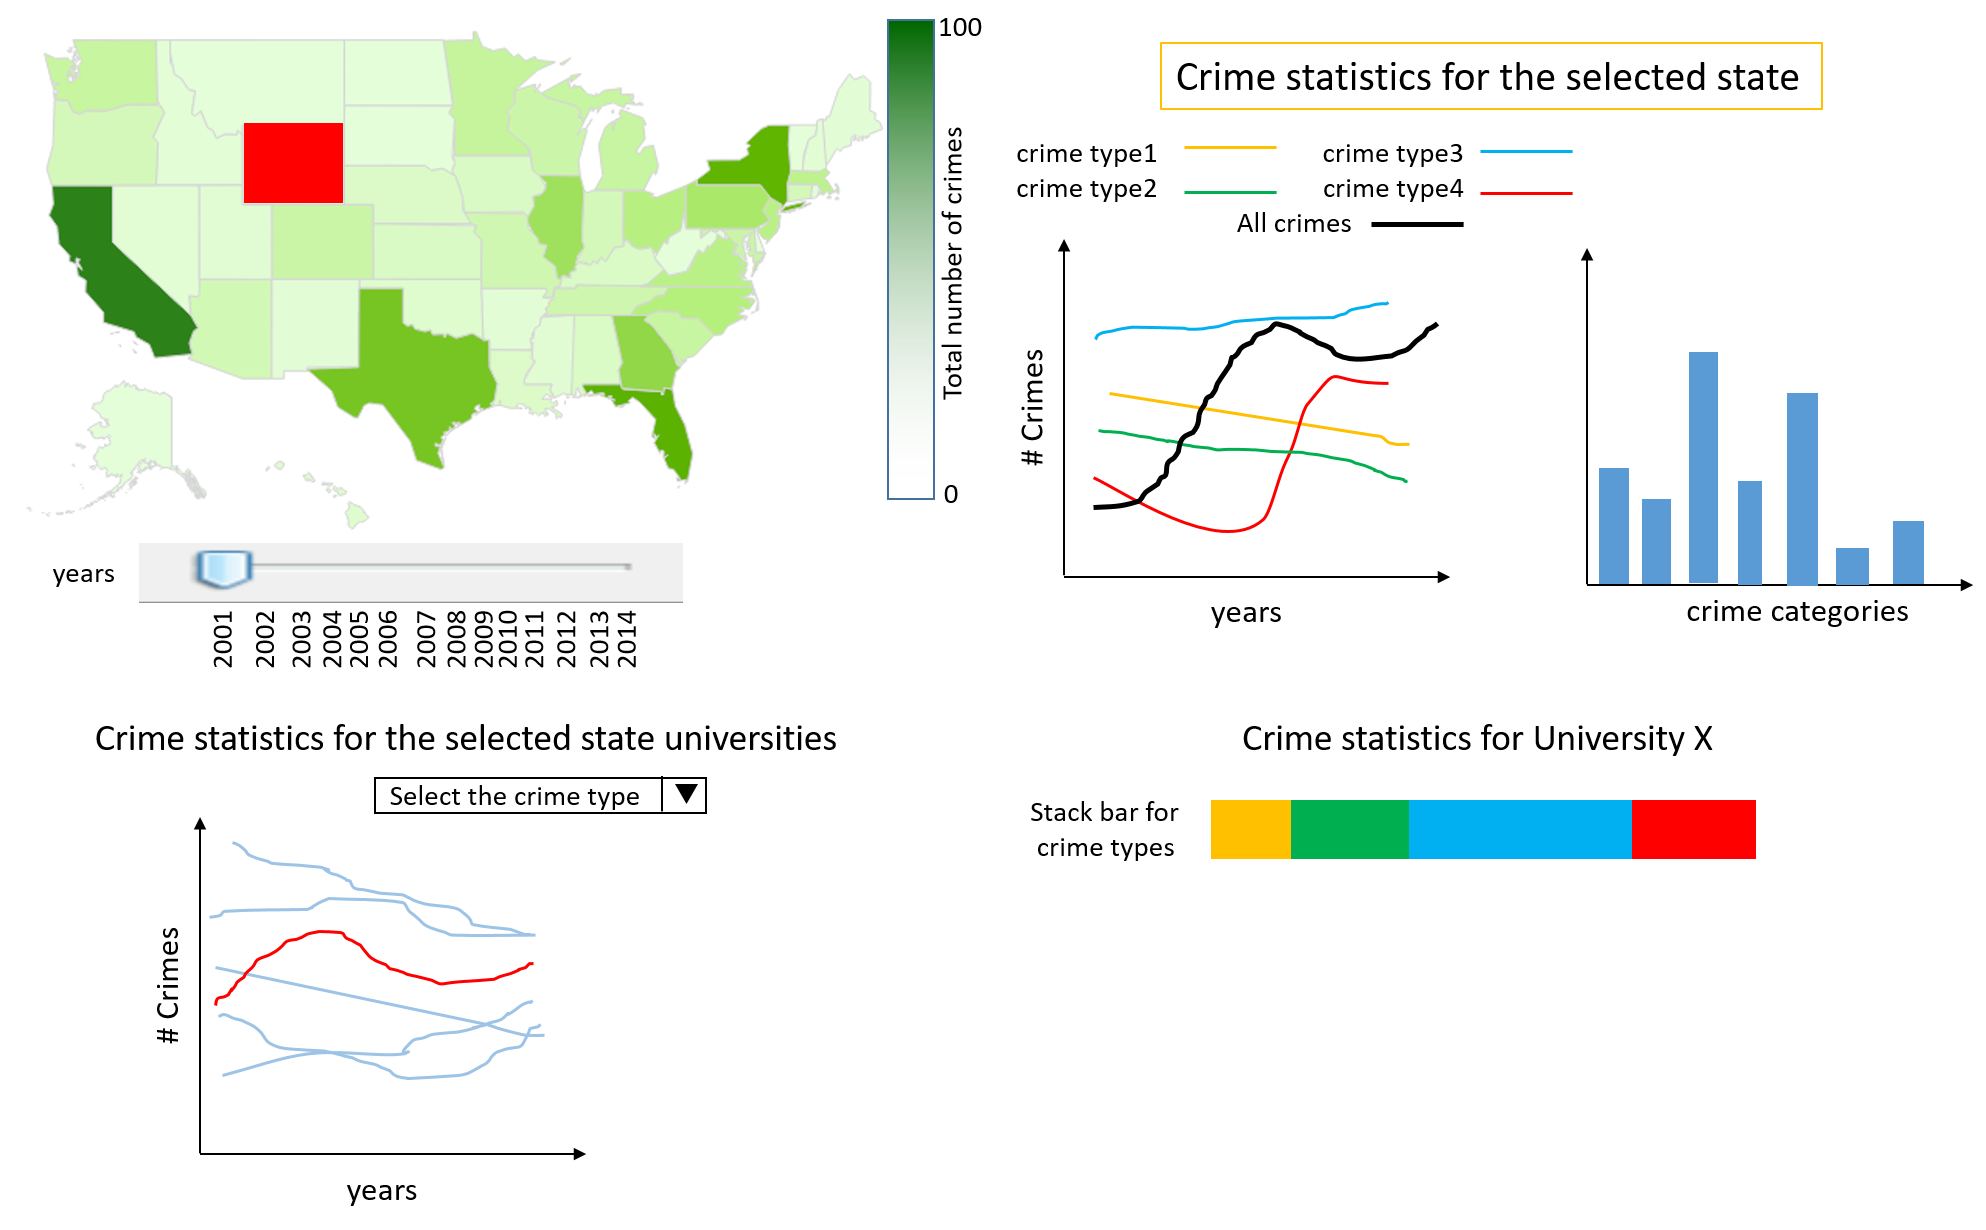
\includegraphics[width=6in]{prot1-5}           
\caption{}
\label{fig:p1-5}
\end{figure}

\begin{figure}[tbph]
   \centering{}
	       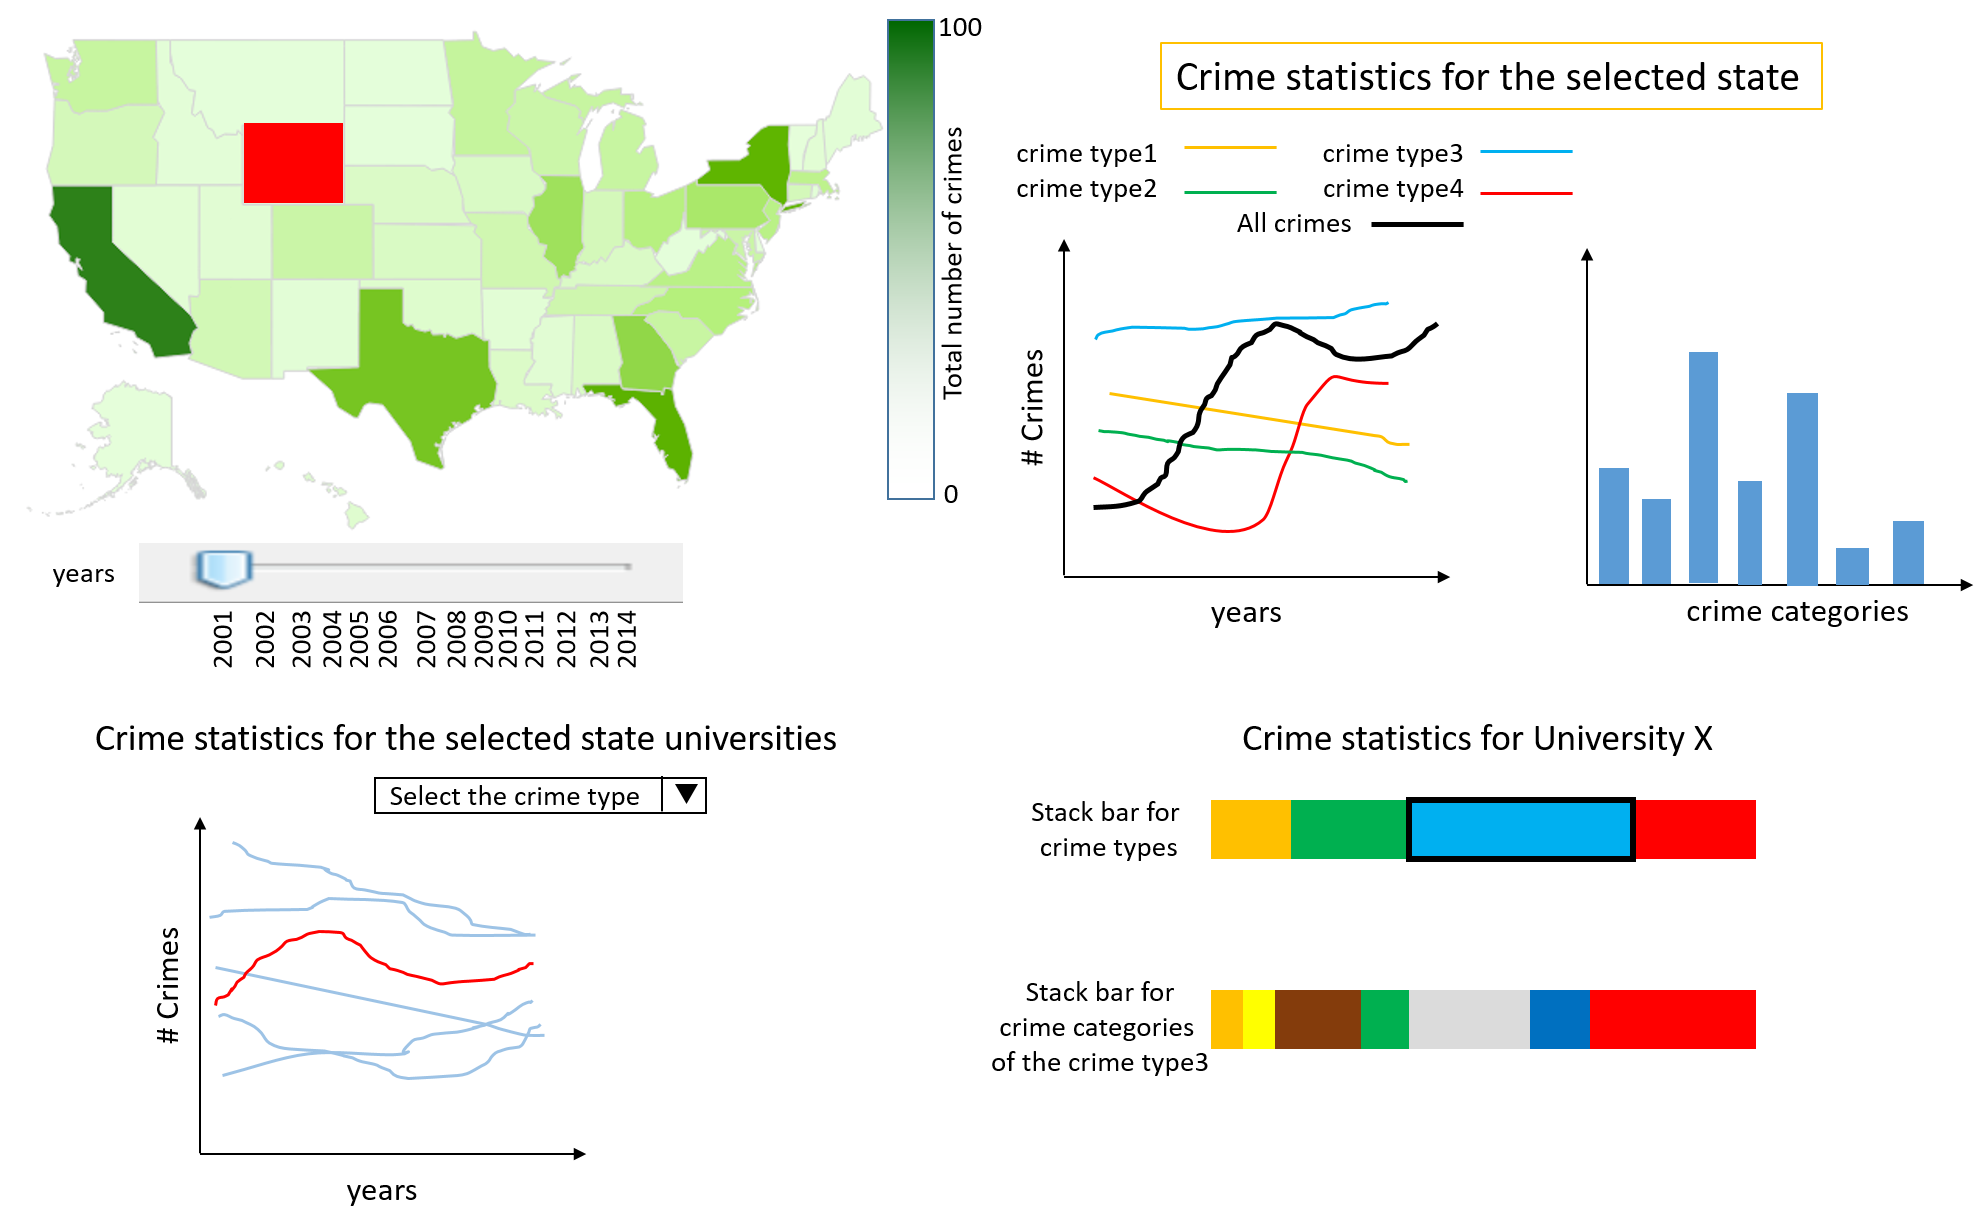
\includegraphics[width=6in]{prot1-6}           
\caption{}
\label{fig:p1-6}
\end{figure}


\subsection{Clustering the data} 
This design will also have the map of the United States. This time we use a scatter plot chart to visualize the data for the whole nation or the selected states (\cref{fig:p3-1}). In this scatter plot, the x-axis represents the total number of crimes while the y-axis represents the number of students. Circles on the scatter plot represent the schools. Therefore, the ratio of the number of crimes to the number of students could be observed on the chart. These information will get updated as the slider for different years gets changed to see how these data get changed over the years. In this prototype in addition to selecting the states, you can use brushing on university circles, to update the selected university line chart and stack bar chart that we had in the first design as well (\cref{fig:p3-2,fig:p1-6}). 


\begin{figure}[tbph]
   \centering{}
	       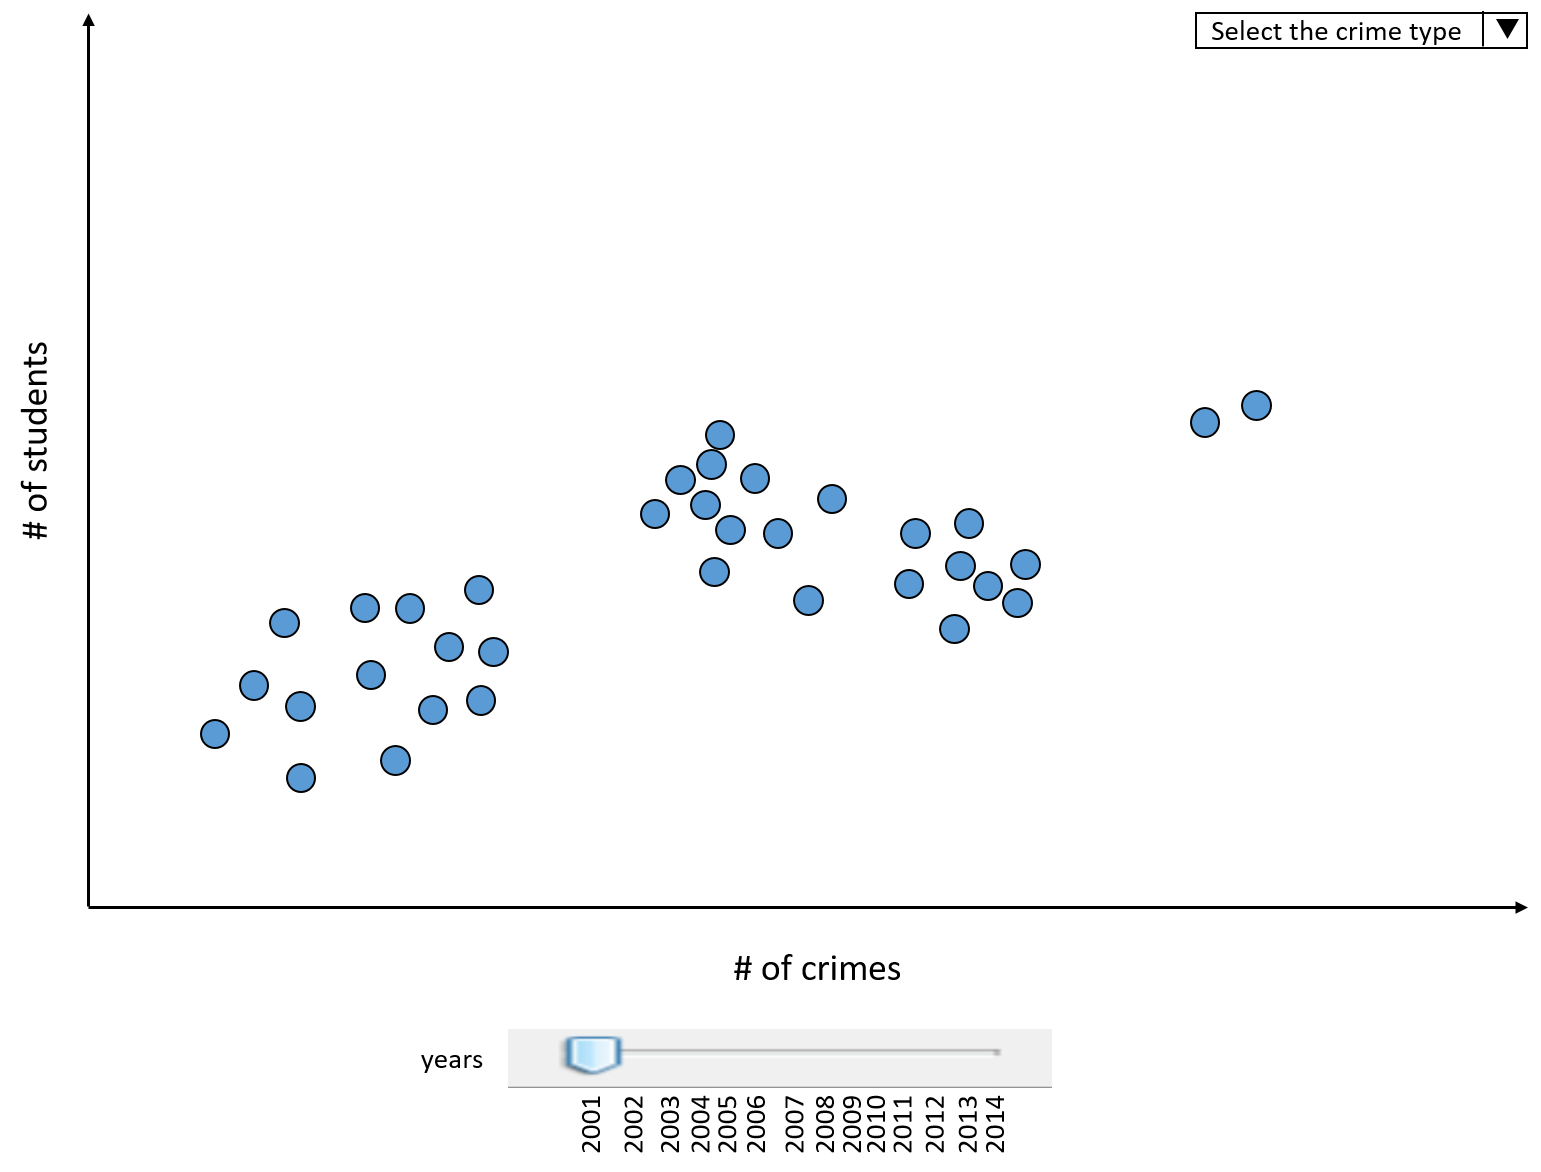
\includegraphics[width=6in]{prot3}           
\caption{}
\label{fig:p3-1}
\end{figure}

\begin{figure}[tbph]
   \centering{}
	       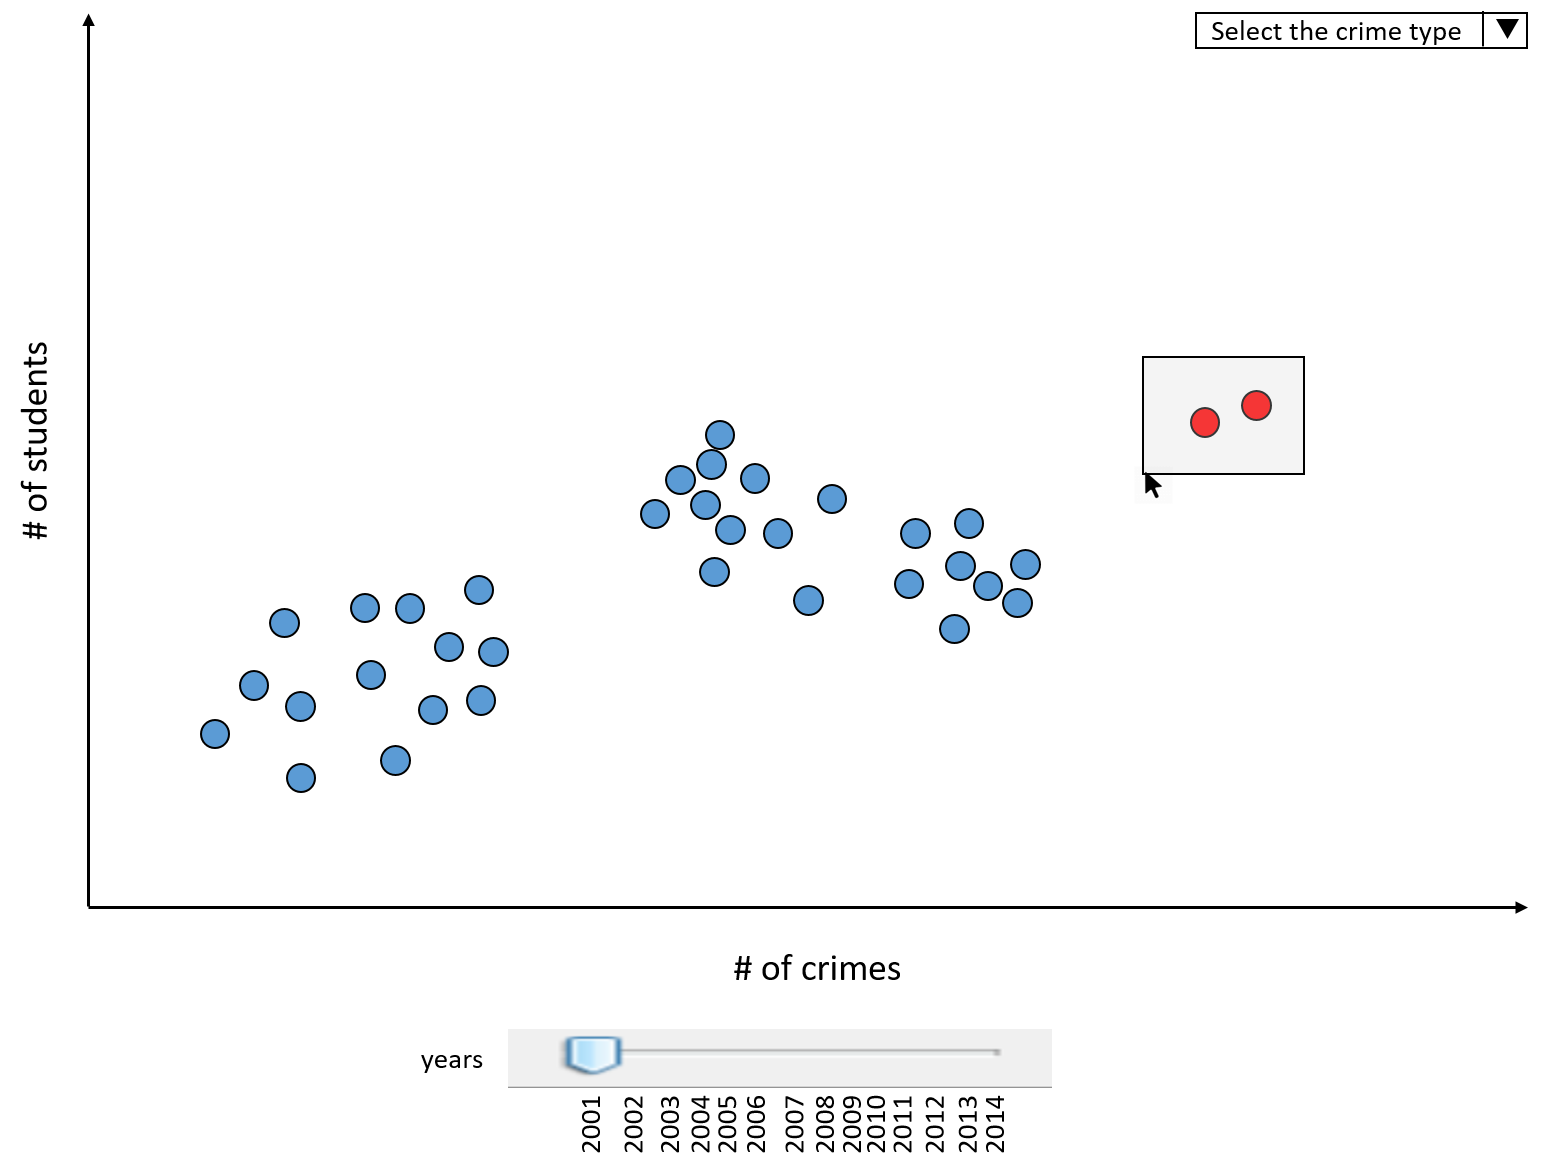
\includegraphics[width=6in]{prot3-2}           
\caption{}
\label{fig:p3-2}
\end{figure}


\subsection{Comparing different types of crime:\label{sec:prot3}} 
In this design instead of a map we display all the universities with circles on the screen. The size of the circles are proportional to the number of the students at each school (\cref{fig:p2-overall}). They are colored using a gradient colormap that uses saturation to show the total number of the crimes at each school over the number of students. The location of the circle gives us a sense of the ratio of four different types crime compared to each other. Namely, if the circle leans on the corner representing criminal offense, the proportion of criminal offense in the corresponding school is higher. Here by hovering over a circle we can highlight it and see the name of te school bold and clear and also the exact number of crimes in that school \cref{fig:p2-1}. There would be a bruch selection to compare statistics of some desired schools in line charts (\cref{fig:p2-2}) and for a selected school on stack barcharts (\cref{fig:p2-3}).

The similarity map visualization presented in class inspired us to think of this design for this prototype. This visualization can be reached at\\ ``http://mariandoerk.de/edgemaps/demo/{\#}music;map;;;".

\begin{figure}[tbph]
   \centering{}
	       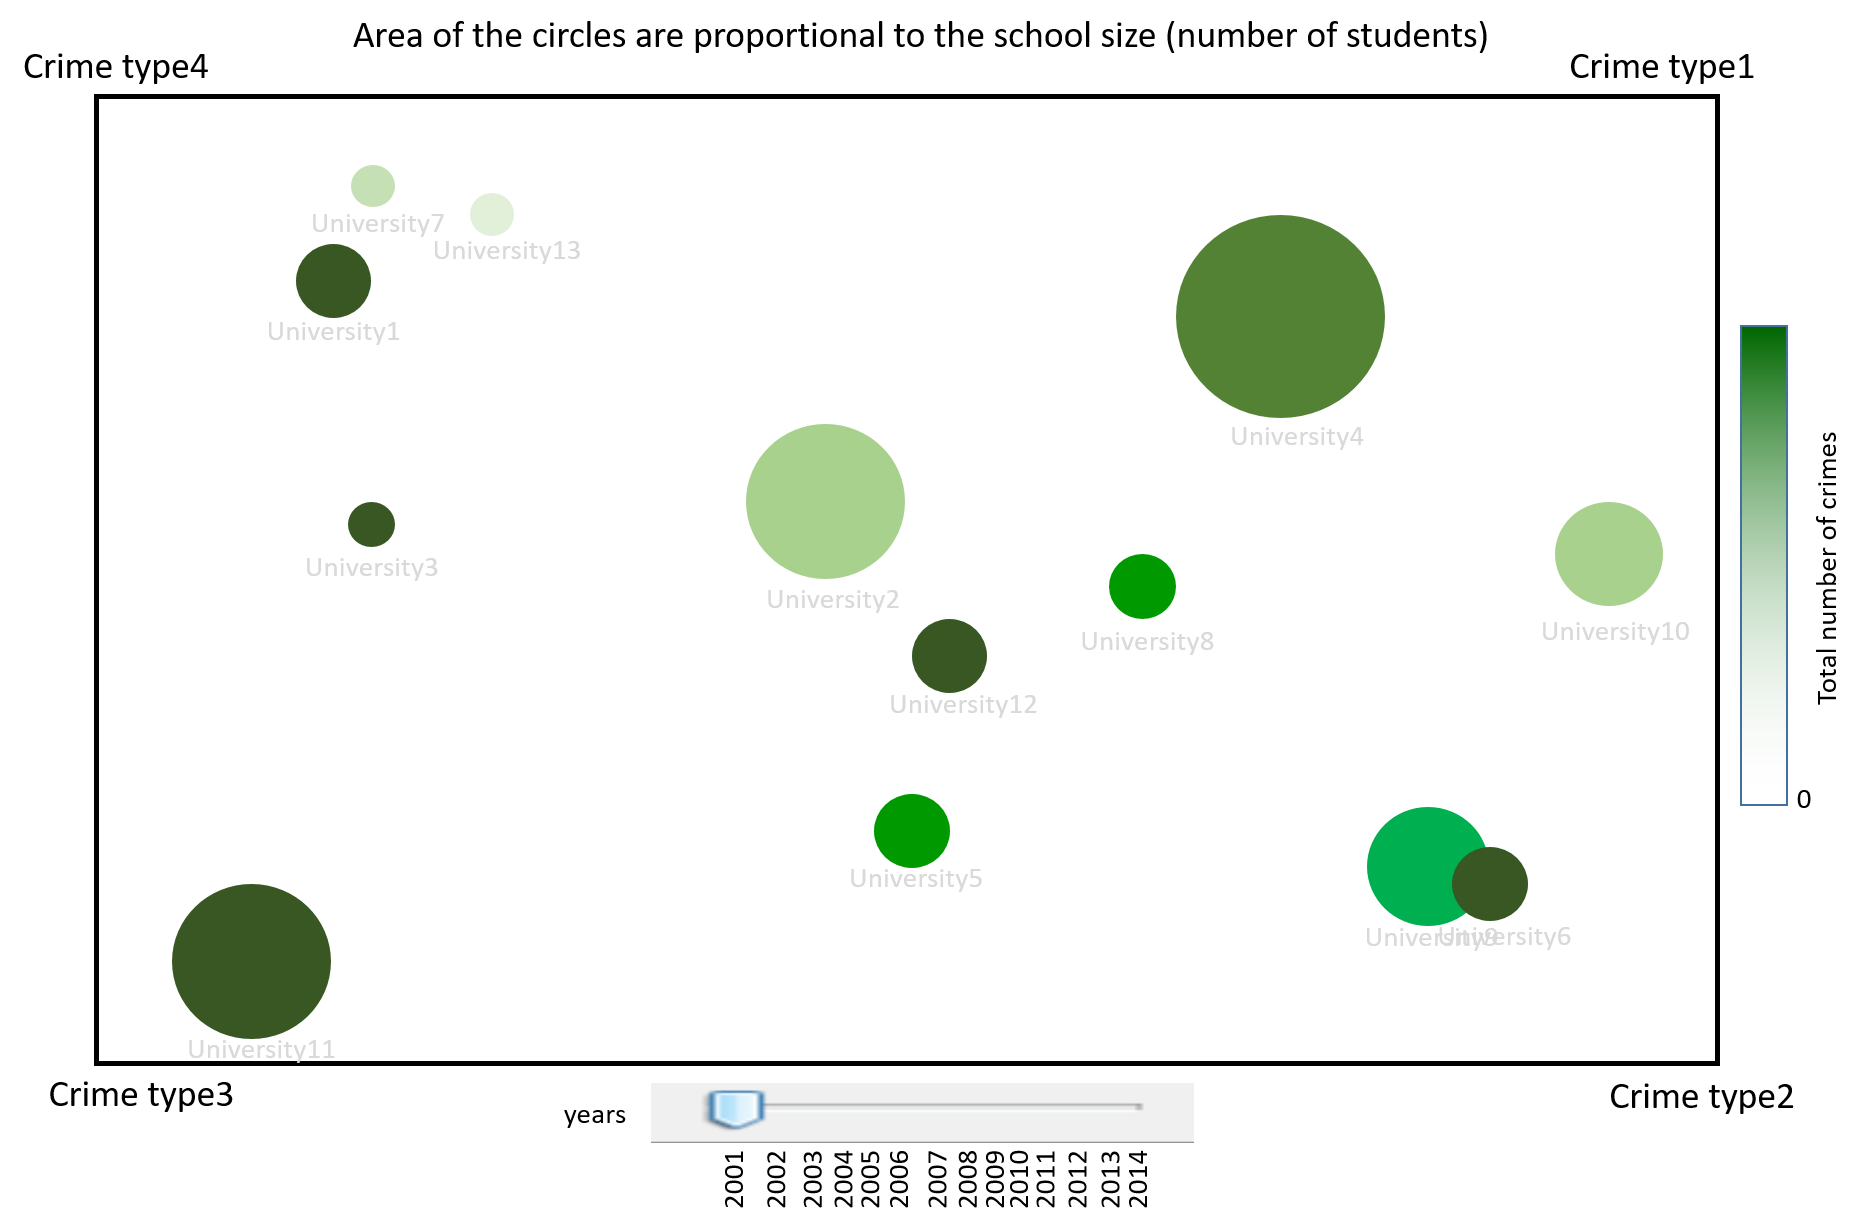
\includegraphics[width=6in]{prot2-overall}           
\caption{}
\label{fig:p2-overall}
\end{figure}

\begin{figure}[tbph]
   \centering{}
	       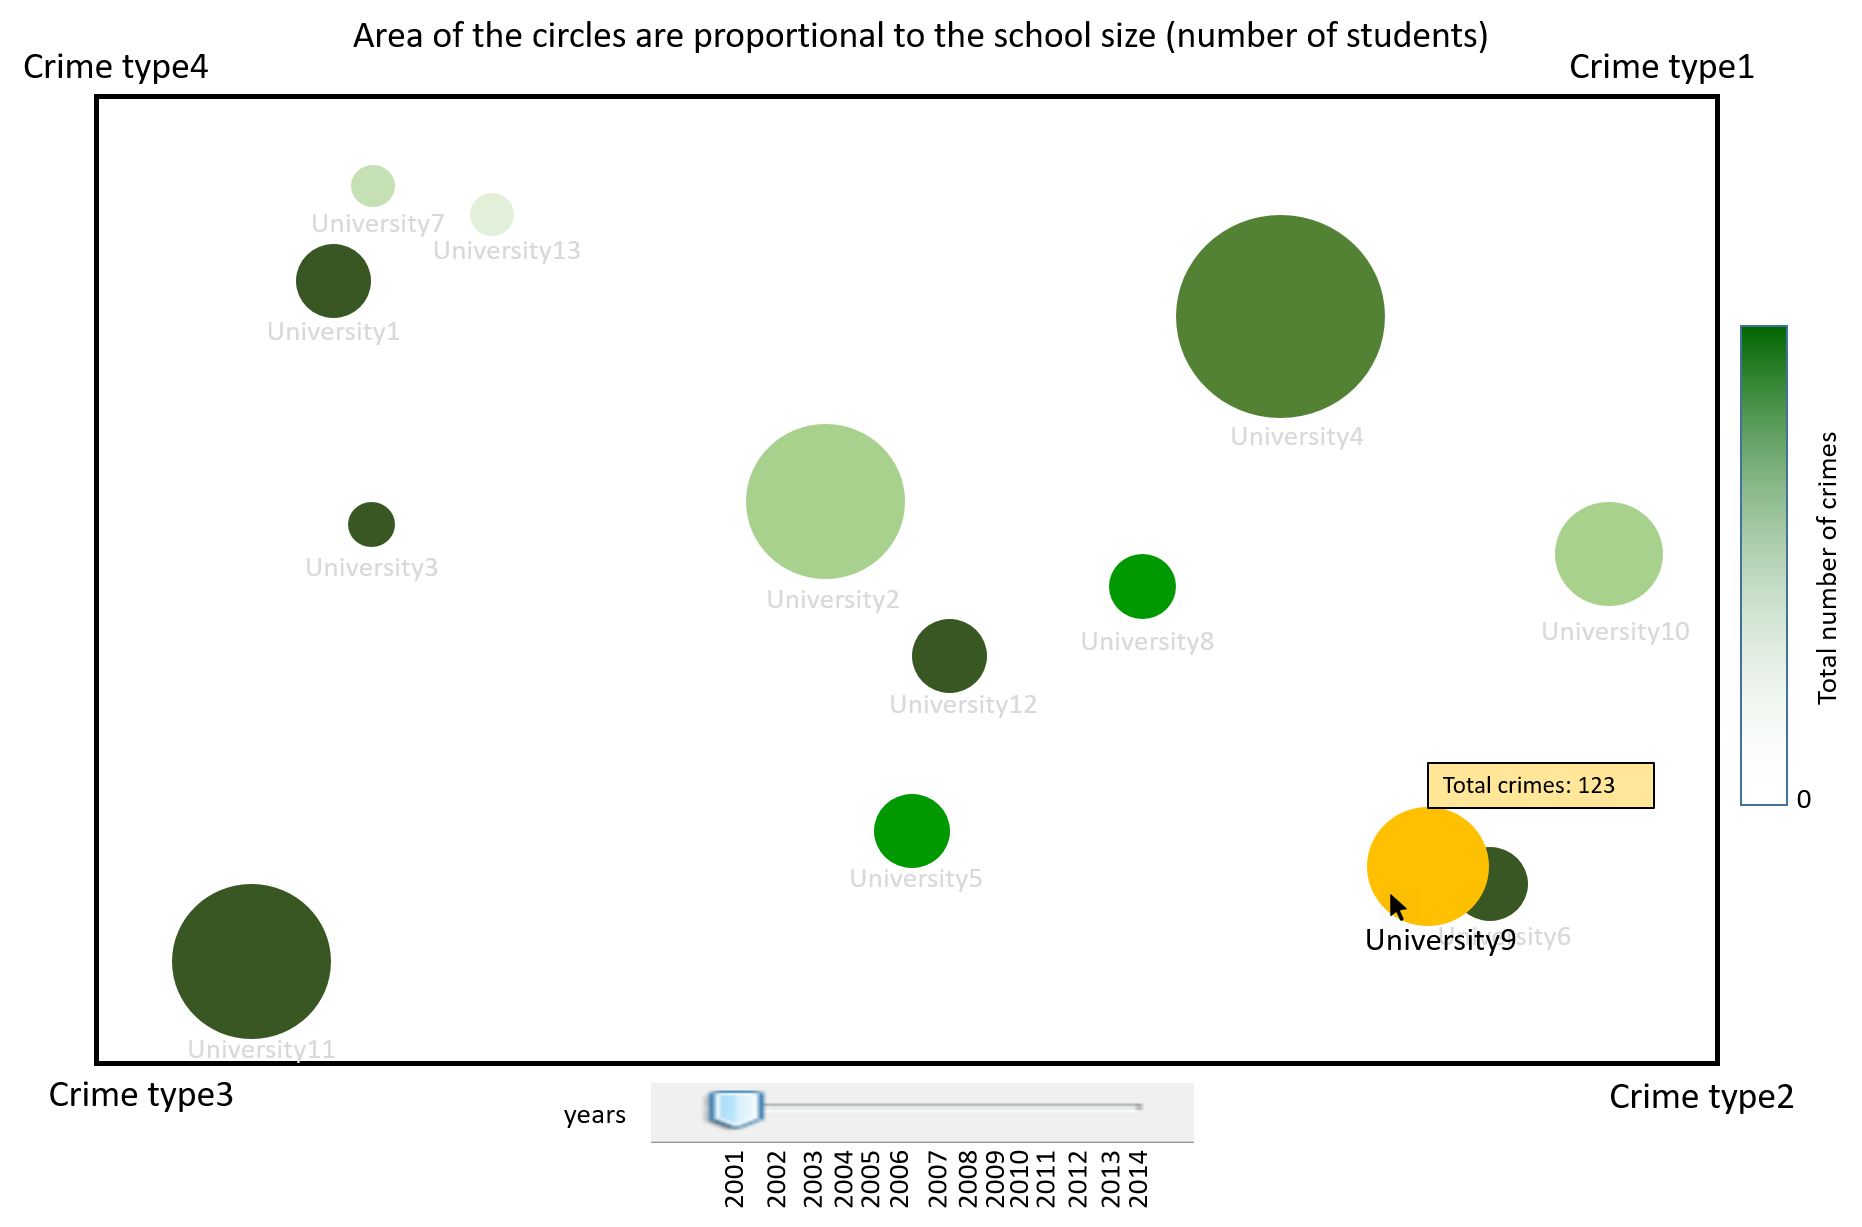
\includegraphics[width=6in]{prot2-1}           
\caption{}
\label{fig:p2-1}
\end{figure}

\begin{figure}[tbph]
   \centering{}
	       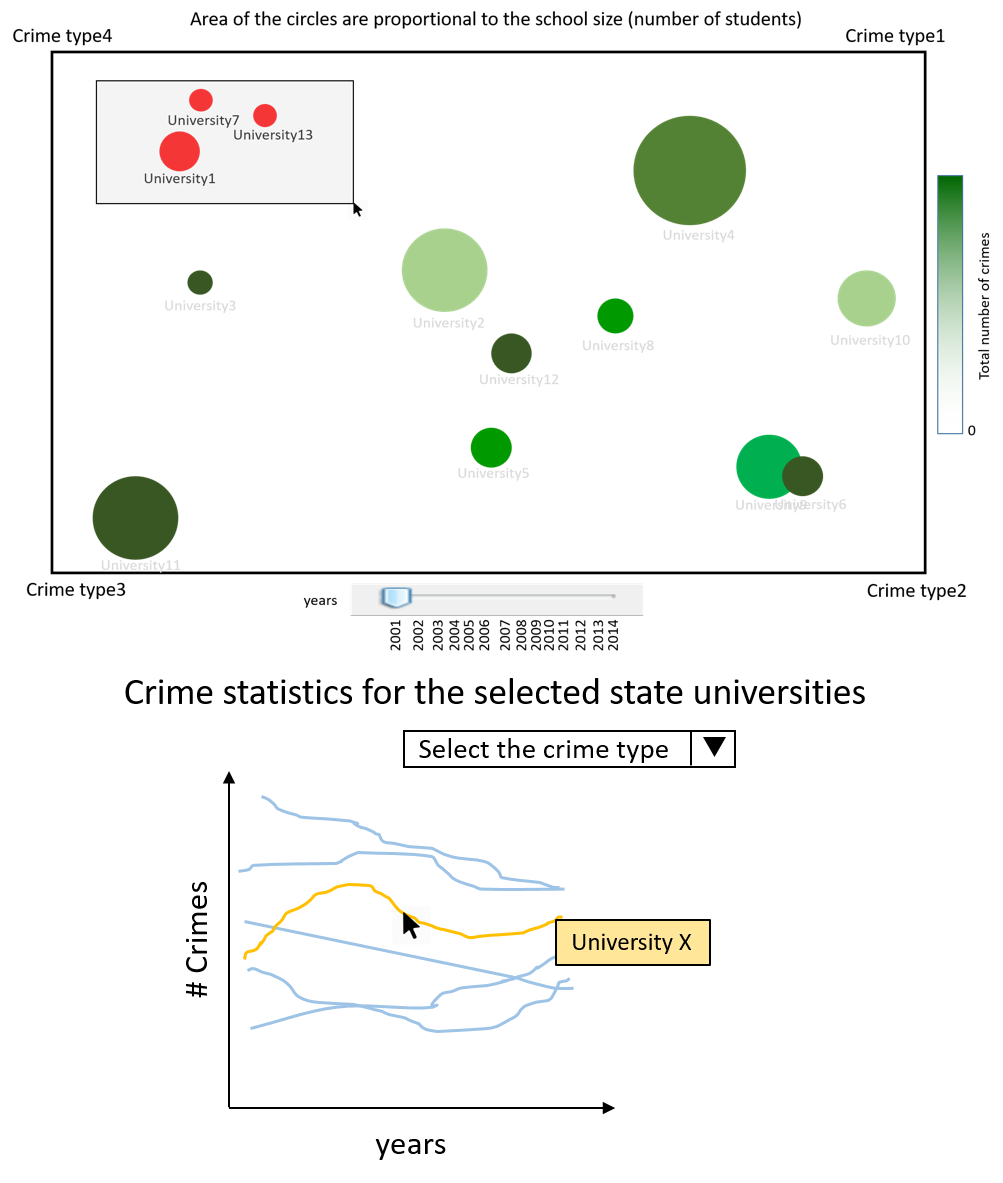
\includegraphics[width=6in]{prot2-2}           
\caption{}
\label{fig:p2-2}
\end{figure}

\begin{figure}[tbph]
   \centering{}
	       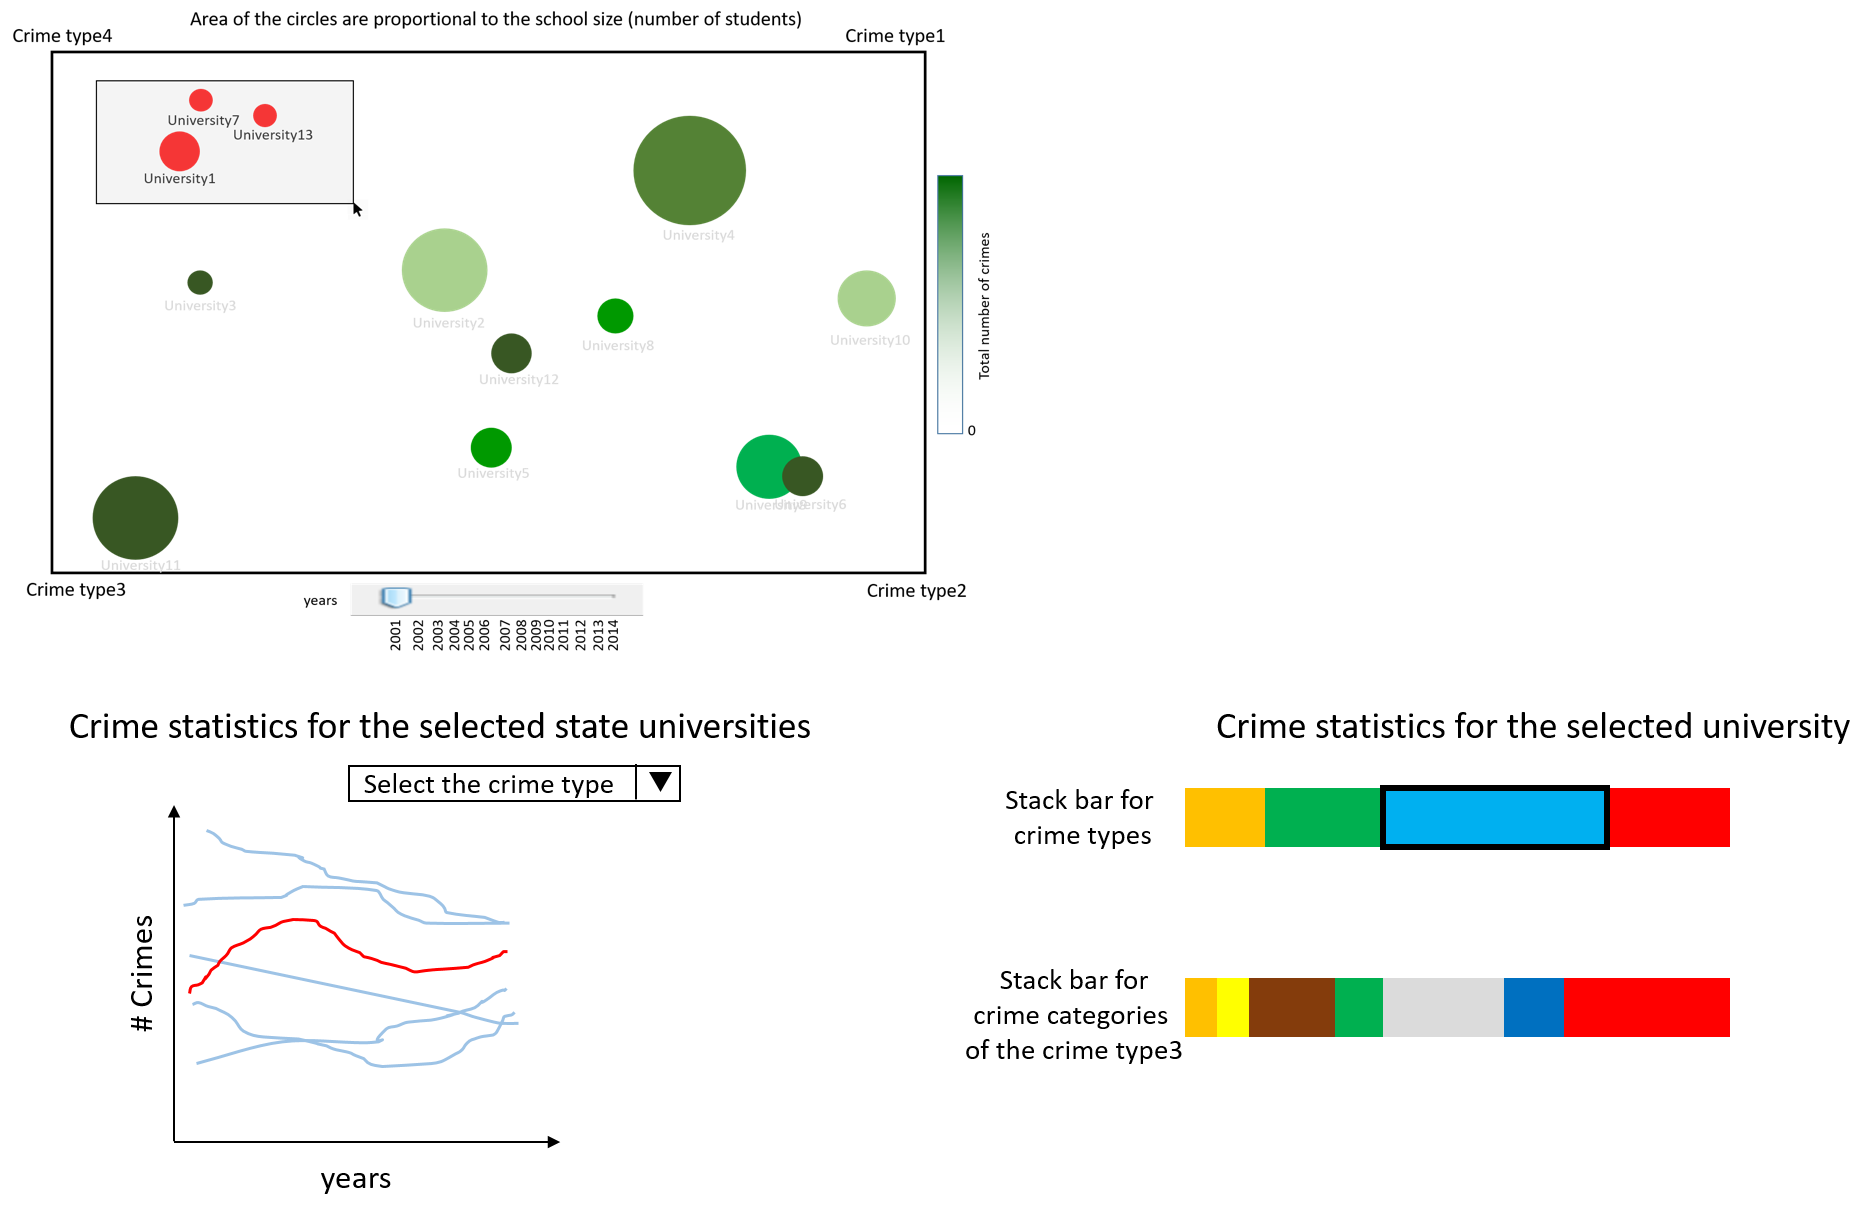
\includegraphics[width=6in]{prot2-3}           
\caption{}
\label{fig:p2-3}
\end{figure}


\subsection{Our selected best design:}

We chose the first design and the third design as our best designs. In both of these designs we use a gradient colormap to qualitatively show a continuous attribute (number of crime per number of students). Then we use position for the most important data (cumber of crime in different categories). We have also used bar charts for separating categories and showing their amount. The stack barcharts are also used to show the percentage of each crime type or category, that uses length, the second best options. These designs, use color (second best choice for categorical attributes) to separates different categories since the spatial region is not available. The third design also uses spatial region to show crime types. 

But there is only one problem with the third design (\cref{fig:p2-overall}), which is there is a probability that the circles of two universities lay on top of each other and make it impossible to separate them. Because of this issue we decided to go with the first prototype (\cref{fig:p1-6}).

\subsection{Issues and critiques}
According to the feedback and critiques we received from our peers and our assigned TA (Yogesh Mishra) there were some issues with our initial designs. Since there may be a lot of  universities in some states like California, the line plot for showing them in \cref{fig:p1-3} may not be a good option to do that. Therefore, we decided to use our third prototype described in \cref{sec:prot3}. But we use it for a selected state here instead of all the universities in US. This will make the universities more distinct.

There was also a suggestion to combine our stack bar charts into one layered donut chart. This can be inspired by the visualization shown at ``https://www.jasondavies.com/coffee-wheel/". In this way we can see the ratio of all the categories at once. We will also get better transitions when selecting one category.  

We also decided to include a line for All of the crimes combined together on the line chart beside the map as you can see in \cref{fig:p1-overall}.


\section{Implementation}
The first view of this visualization is the map of United states. We can interact with the map and update other charts from here. It was crucial to implement this part correctly and make it ready for smooth transitions and synchronizations.
For this part we used a topo-jason file to draw the US map which included state ID's. We passed the state abbreviations to drawn states on the map to have access to them later. We also attached a tool-tip which pops up when the mouse hovers over a state showing general information about it. A range input is implemented to handle the time slider below the map. This allows us to move across different years and access the related data. There is also an "onclick" event for each state. The user can click a state to select it and see its corresponding data visualized on rest of the charts. It all could be seen in \cref{fig:map}.

\begin{figure}[H]
   \centering{}
	       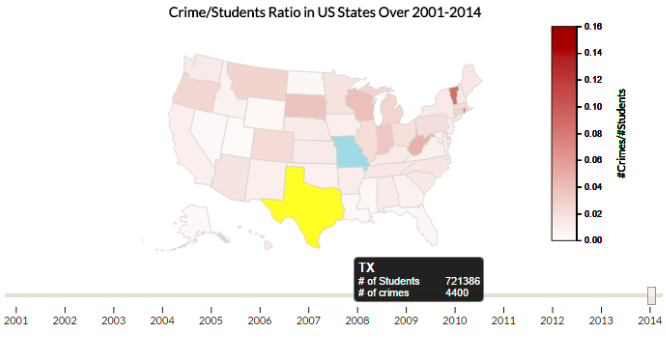
\includegraphics[width=5in]{map.PNG}           
\caption{}
\label{fig:map}
\end{figure}



By choosing a state on the map, two new charts would get updated. The first one is a line chart in which each line displays the stats for one type of crime in the selected state during all the years the survey has been conducted. By clicking on each one of the lines, a bar chart will appear showing the number of crimes committed in each category included in the selected type of crime. Dues to lack of space, the name of each category is displayed in a tooltip whenever mouse hovers over one of the bars. An example is shown in \cref{fig:charts}.
\begin{figure}[H]
   \centering{}
	       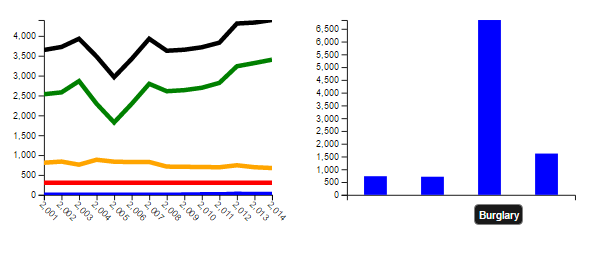
\includegraphics[width=5in]{chart.PNG}           
\caption{}
\label{fig:charts}
\end{figure}

The second chart which get updated after selecting s state is the ratio Chart. The institutes in the selected state would be displayed on a rectangular chart, each being represented by a circle. In this chart, each corner represents one of the four types of crimes. And as a crime type has a larger role in the total number of crimes in an institute, the said institute would be placed closer to the corresponding corner. In this chart the size of each university is displayed via the size of its circle. Also, color saturation is used to display the ratio of number of crimes in each institute to its number of students. An example could be seen in \cref{fig:ratio}.

\begin{figure}[H]
   \centering{}
	       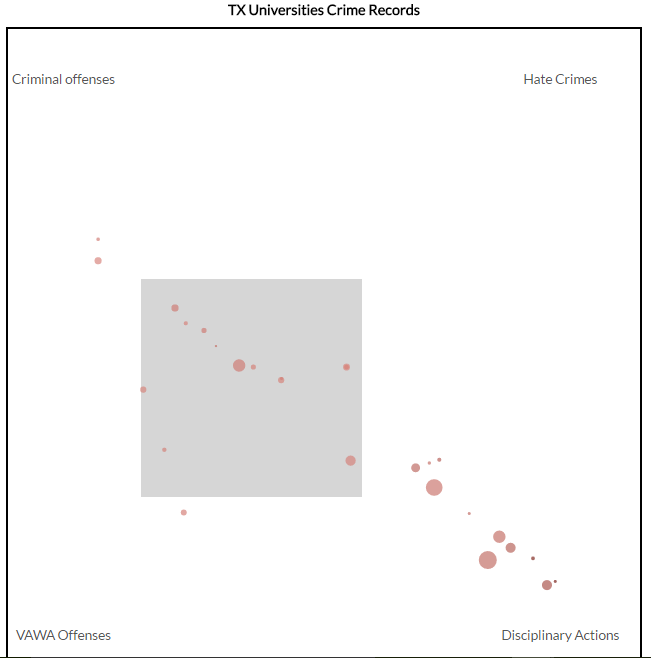
\includegraphics[width=4in]{ratio.PNG}           
\caption{}
\label{fig:ratio}
\end{figure}

By clicking on one of the circles on the ratio chart, the SunBurstTree chart would pop up displaying the full crime stats for the university which has been selected. This chart looks like a layered donut in which, the first layer represents the crime types and the second one represents the categories in each type. Also, by clicking on a a specific type of crime, the chart gets updated and as shown in \cref{fig:donut} and by clicking on the inner circle it goes back to its initial shape.

\begin{figure}[H]
   \centering{}
	       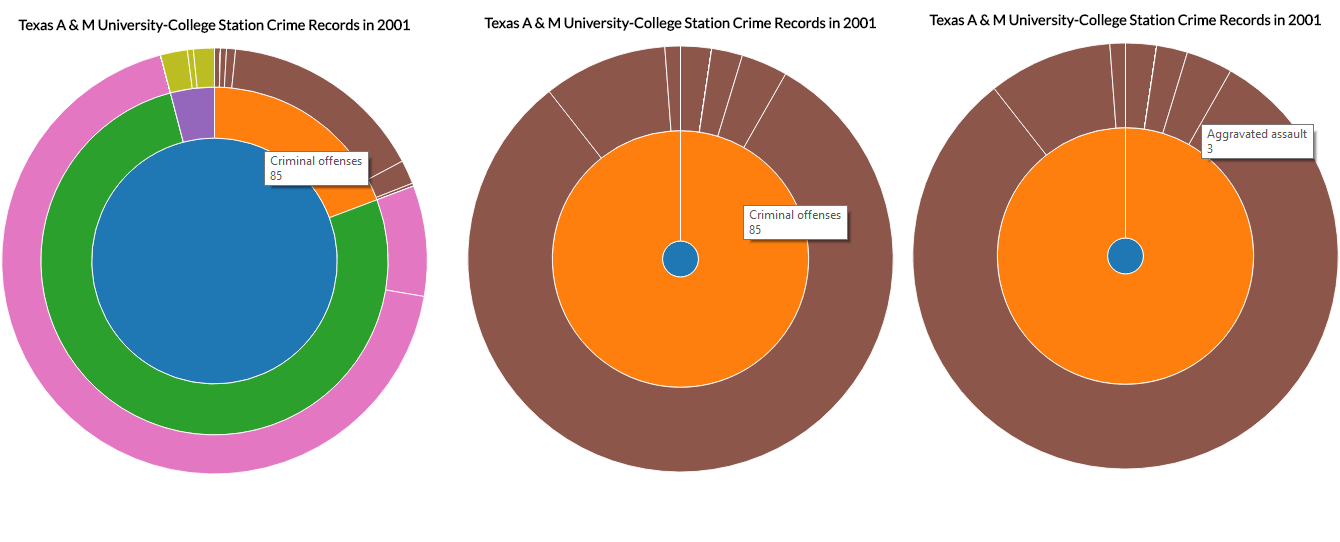
\includegraphics[width=7in]{donut.PNG}           
\caption{}
\label{fig:donut}
\end{figure}

By selecting a set of universities on the ratio chart via brush, the comparison table gets updated. As the name suggest, the goal of this table is to compare crime statistics in different schools \cref{fig:donut}:

\begin{figure}[H]
   \centering{}
	       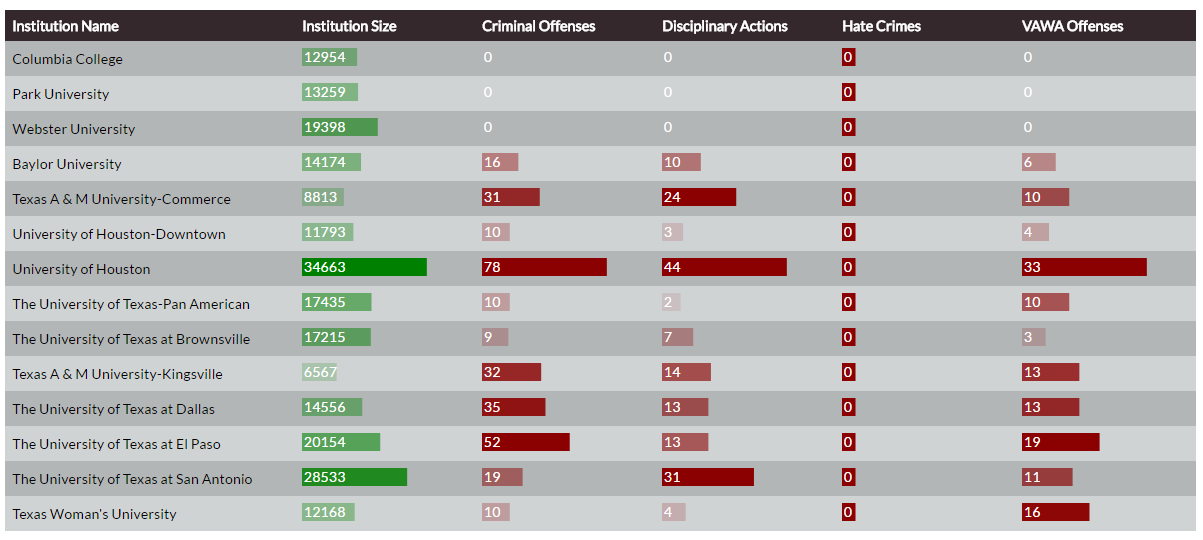
\includegraphics[width=6in]{table.PNG}        
\caption{}
\label{fig:donut}
\end{figure}

\section{Evaluation}



 

%----------------------------------------------------------------------------------------

\end{document}